\documentclass[11pt,a4paper]{article}

%francais
\usepackage[utf8]{inputenc}   
\usepackage[T1]{fontenc}           
\usepackage[francais]{babel}  

%2col/présentation de la page
\usepackage[hmarginratio=1:1,margin=20mm,columnsep=20pt]{geometry}
       
%images
\usepackage{float}
\usepackage{graphicx}
\usepackage{caption}
\addto\captionsfrench{\renewcommand{\figurename}{\textsc{Image}}}

%liens
\usepackage{hyperref}
\hypersetup{breaklinks=true}
\urlstyle{same}

%joli
\usepackage{enumerate}
\usepackage{enumitem}
\setitemize{label=$\bullet$}%,leftmargin=*,topsep=0pt,noitemsep,parsep=0pt}
\usepackage{amsmath,amssymb,amsfonts}
\usepackage{xcolor}
\usepackage[lighttt]{lmodern}

%tableaux
\usepackage{makecell}
\renewcommand\theadalign{cb}
\renewcommand\theadfont{\bfseries}
\renewcommand\theadgape{\Gape[4pt]}
\renewcommand\cellgape{\Gape[4pt]}

%schémas
\usepackage{tikz}
\usetikzlibrary{positioning}

%subdivisions
\usepackage{titlesec}
%\titleformat{\section}{\normalfont\bfseries}{}{1pt}{\normalfont\bfseries}{}
%subsubsub section
\usepackage{titlesec}

%code
\usepackage{listings}
\usepackage{adjustbox}
%environnement
\newenvironment{code}{
\footnotesize%
\ttfamily%
\begin{adjustwidth}{2.2em}{0em}%
}
{%
\end{adjustwidth}%
\normalfont%
\normalsize%
}

%en-têtes
\usepackage{fancyhdr}
% style première page
\fancypagestyle{plain}{%
  \fancyhf{}%
\fancyfoot[C]{\thepage}
% Line at the header invisible
  \renewcommand{\headrulewidth}{0pt}
}
%style autres pages
\pagestyle{fancy}%
  \fancyhf{}%

%subsubsubsection command
\setcounter{secnumdepth}{4}
\setcounter{tocdepth}{4}

%formatage des titres de paragraphes comme subsubsubsection
\titleformat{\paragraph}
{\normalfont\normalsize\bfseries}{\theparagraph}{1em}{}
\titlespacing*{\paragraph}
{0pt}{3.25ex plus 1ex minus .2ex}{1.5ex plus .2ex}


%%%%%%%%%%%% :TODO: : noms
\fancyhead[R]{\textsc{Couvreur} Alexis}
%%%%%%%%%%%% :TODO: : titre
\fancyhead[L]{\textsc{Projet d'ArchiOSHPC}}
\fancyfoot[C]{\thepage}%


\setlength\parindent{9pt}
\pagenumbering{arabic}

\begin{document}


\pagestyle{empty}

\begin{center}
{\LARGE Projet en architecture des processeurs hautes
performances et programmation efficace} \\[.8cm]
{\large \textsc{Couvreur} Alexis \quad} \\[2cm]
\end{center}

\tableofcontents


\clearpage

\section{Description de l'environnement expérimental}

\pagestyle{fancy}

\subsection{Description de l'environnement matériel}
La machine Linux utilisée est un raspberry pi 3b et dispose de quatre processeurs superscalaires ARM Cortex-A53 cadencés à une fréquence de 1.2GHz au maximum et d'une mémoire RAM de 1GB LPDDR2 (900 MHz) qui supporte l'architecture ARMv8, cependant notre matériel utilise l'architecture ARMv7 dessus.
L'environnement détecte un socket avec quatre cœurs physiques, il n'y a donc pas d'Hyperthreading.
\paragraph*{Architecture}
Il s'agit donc d'un processeur RISC qui implémente le jeu d'instructions ARMv7 32-bit.

\paragraph*{Microarchitecture} 
\begin{itemize}
\item Un pipeline de 8 étage avec deux instructions par cycle ;
\item cache L1 32Ko instructions et 32Ko données ;
\item cache L2 512Ko ;
\item pas de cache L3 ;
\item taille ligne cache de 64 octets ;
\item les caches sont à 4 voies associatives
\item L1 a une interface d'écriture vers L2 de 256 bits ;
\item L1 a une interface de lecture vers L2 de 128 bits ;
\item TLB de 512 entrées ;
\item présence d'une unité de prédiction de branchement ;
\item présence d'une unité d'exécution out-of-order ;
\item présence d'une unité de renommage de registres ;
\end{itemize}

Le service DVS à été désactivé, les processeurs sont cadencés à 1.2GHz en permanence.
Je n'ai pas réussi à désactiver la prédiction de branchement, il faut modifier le registre C15 lors du boot cependant je n'y suis pas parvenu.

\subsection{Description de l'environnement logiciel}

Il s'agit d'un environnement sous \texttt{Raspbian GNU/Linux version 8 (Jessie) noyau version 4.4.43-v7+}.\\
Le compilateur GCC utilisée est \texttt{gcc (Raspbian 4.9.2-10) 4.9.2} avec aucune options de compilation, on ne souhaite pas utiliser O1 ou plus étant donné que l'on veut que le code soit exécuté de manière séquentielle, et exactement de la manière dont le code est écrit.\\
Les mesures du temps sont effectuées via \texttt{clock\_gettime} pour une précision à la nanoseconde en utilisant un référentiel monotonic.
\pagebreak
\section{Configuration de la machine pendant les expériences}

La machine lors des expériences est sans interface graphique, mode console seulement, avec 3 à 4 processus utilisateur en moyenne (en enlevant les processus bash et celui de la commande ps).\\
Comme dit plus haut, la fréquence d'horloge est 1.2GHz en permanence.\\
Ainsi on a une charge minimale, avec un travail de la part du processeur au maximum. Pour récolter les résultats j'ai donc détourner la sortie vers un fichier d'output, cela n'impacte pas les données car les calculs sont fait dans une itération interne au processus. Les difficultés expérimentales étaient de savoir si les données représentaient vraiment ce que l'on attendait des exercices, j'ai donc dû m'y reprendre à plusieurs fois pour vérifier certains effets en changeant les paramètres, au début le taille max était égale à 2 * la taille du niveau de cache maximal + 1 octet. \\Mais finalement j'ai opté pour que cela soit égal à 3 * la taille du niveau de cache maximal pour bien voir des différences, et au final j'en suis plutôt satisfait.

\section{Exercice 1}
Cet exercice cherche à mettre en évidence les accélérations que permettent les différents niveaux de cache, il s'agira des caches L1 et L2 sur cette configuration. \\
On sait que le cache L1 a une valeur de 32Ko et le L2 a une valeur de 512Ko, que le cache L1 est un cache propre à un seul cœur tandis que le cache L2 est partagé.\\
Nous pouvons alors émettre l'hypothèse suivante : le temps d'accès aux données dans le cache L1 sera le plus bas, dépassé les 32Ko de données, le cache L2 prendra le relais.

\begin{center}
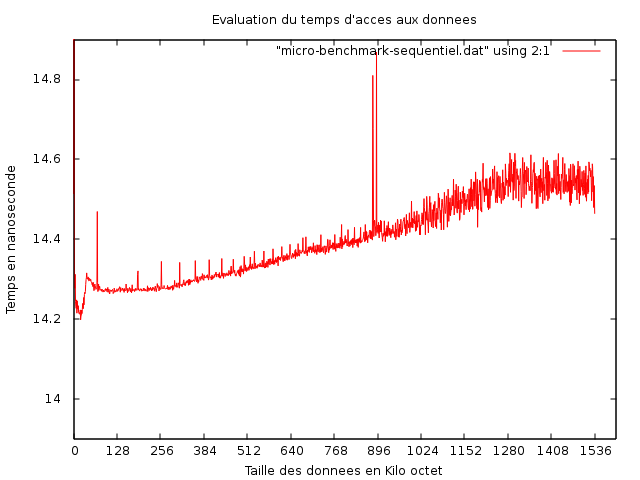
\includegraphics[keepaspectratio=true,width=\linewidth]{Exercice1/micro-benchmark-sequentiel.png}
\captionof{figure}{Évaluation du temps d'accès moyen aux données}
\end{center}
\pagebreak
Notre hypothèse est confirmée et on remarque aussi certains motifs apparaître, tel que des pics à intervalles réguliers d'environ 32Ko d'écart ! Je pense qu'il s'agit d'un défaut de cache L1 qui demande donc au cache L2 de prendre le relais.\\
On remarque en plus aux alentours de 900 Ko, un gros pic et ensuite le temps d'accès devient très instable en augmentant plus qu'avant, je pense qu'ici le cache L2 ne suffit plus à traiter autant de données et donc que le fait de vider le cache et réécrire dedans fait évidemment augmenter le temps d'accès.\\
Ici le temps d'accès est compris entre 14,20 et 14,95 nanosecondes.\\
J'ai reproduit cette expérience sur un seul processeur avec la commande taskset pour voir si le parallélisme influence beaucoup ce benchmark, je fais l'hypothèse que non car il y a très peu de calcul à paralléliser car il s'agit principalement d'accès mémoire.
\begin{center}
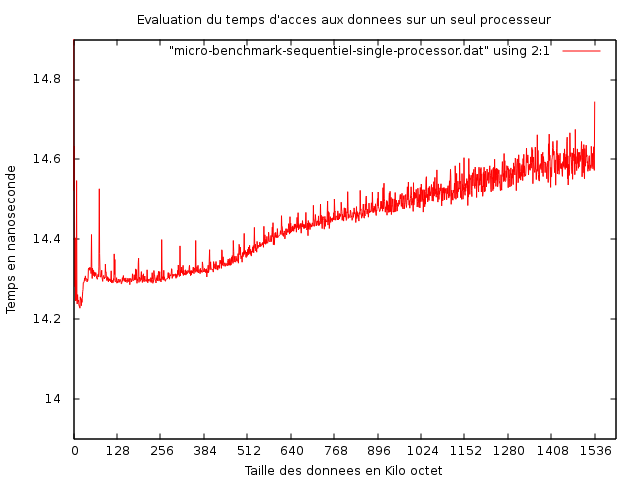
\includegraphics[keepaspectratio=true,width=\linewidth]{Exercice1/micro-benchmark-sequentiel-single-processor.png}
\captionof{figure}{\textsc{Évaluation du temps d'accès moyen aux données} sur un seul processeur}
\end{center}
On perçoit quelques changements, notamment la disparition du pic mais cela reste globalement la même chose.\\
Le temps d'accès est compris entre 14,22 et 14,95 nanosecondes.

\pagebreak
\section{Exercice 2}

Cet exercice est relativement identique au premier à l'exception que l'accès aux différentes données ne doit pas se faire de manière contigu ! Pour cela, on va se baser sur la taille de notre ligne du cache, cette ligne est chargée à chaque fois qu'une donnée est demandée. Évidemment comme la donnée n'a pas forcément la même taille que la ligne elle même la ligne peut charger les données contigus dans la mémoire ! Ainsi on chargera des données qui ont un écart dans la mémoire de la taille de la ligne de cache.\\
On peux alors émettre l'hypothèse suivante : on aura un courbe croissante qui se stabilisera à son débit maximum.

\begin{center}
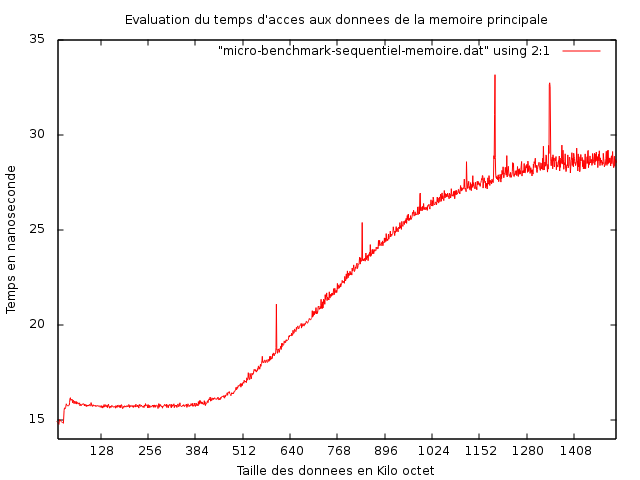
\includegraphics[keepaspectratio=true,width=\linewidth]{Exercice2/micro-benchmark-sequentiel-memoire.png}
\captionof{figure} {Évaluation du temps d'accès moyen aux données de la mémoire principale}
\end{center}
On remarque donc que notre hypothèse est confirmée, si l'on compare ce graphique à celui de l'exercice 1 la différence est immédiate. Le temps d'accès est compris entre 14,8 et 30 nanosecondes.

J'ai reproduit cette expérience sur un seul processeur avec la commande taskset pour voir si le parallélisme influence beaucoup ce benchmark,même hyspothèse qu'à l'exercice 1 : très peu de parallélisme donc peu de variation.\\
\begin{center}
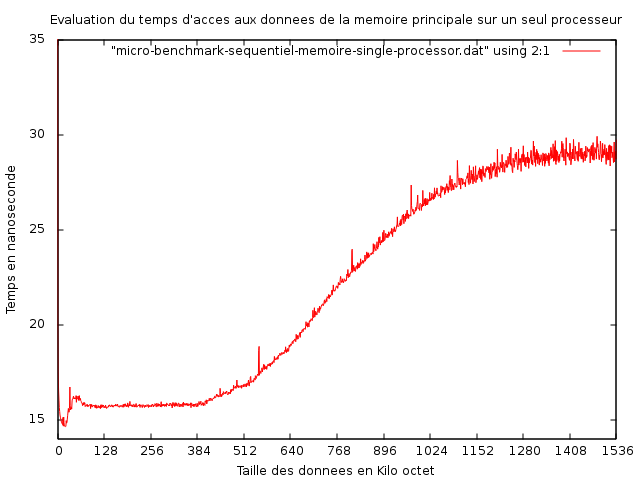
\includegraphics[keepaspectratio=true,width=\linewidth]{Exercice2/micro-benchmark-sequentiel-memoire-single-processor.png}
\captionof{figure} {Évaluation du temps d'accès moyen aux données de la mémoire principale sur un seul processeur}
\end{center}
On remarque bien que les graphes sont très ressemblant. Le temps d'accès est aussi compris entre 14,8 et 30 nanosecondes.
\pagebreak
\section{Exercice 5}
L'outil calibrator est plus puissant pour plusieurs raisons, il implémente plusieurs mécanismes permettant de contourner des optimisations de branchement (prédictions, out-of-order, etc.) et se base sur le constat de ses résultats et non sur des données matériels comme la taille du cache L1, la taille du cache L2 ou encore la taille d'une ligne de cache. Il va déduire ces données par rapport aux résultats des calculs effectués.

\section{Compréhension personnelle}

Ma compréhension personnelle sur ce projet ne s'étale pas grandement en dehors du cours, certains mécanismes se sont concrétisés et donc ma compréhension de ceux-ci est plus clair.

\section{Conclusion}
Au cours de ce projet j'ai dû effectuer diverses expériences, traiter le résultat et l'interpréter. La phase d'interprétation n'aurait pas été possible sans les cours d'architecture qui ont permis l'appréhension de beaucoup de concepts lors de mes recherches. \\Je pense que cela m'a permis de concrétiser l'étude d'un processeur, lors de mes recherches, j'ai pu me renseigner sur le processeur de ma machine sur la documentation de chez ARM (\href{http://infocenter.arm.com/help/topic/com.arm.doc.ddi0500e/BABJBFEJ.html}{lien vers la documentation du processeur Cortex-A53}) et ainsi comprendre l'implémentation du cache, les diverses technologie présentes et en déduire certains effets.\\
Ce projet m'a beaucoup plu car j'y ai notamment pu découvrir l'architecture de mon raspberry pi ! Faisant des projets de temps en temps dessus, je réfléchirai plus sur la façon de programmer certaines choses pour optimiser au mieux les performances.

\end{document}
